\documentclass[twocolumn,11pt]{article}
\usepackage[margin=1in]{geometry}
\usepackage{graphicx}
\usepackage{amsmath}
\usepackage{amssymb}
\usepackage{hyperref}
\usepackage{natbib}
\usepackage{booktabs}
\usepackage{float}
\usepackage{tabularx}

\title{Citation Fidelity in Social Media: How Bluesky Users Represent ``AI Models Collapse When Trained on Recursively Generated Data''}

\author{Anonymous}

\date{\today}

\begin{document}

\maketitle

\begin{abstract}
The 2024 Nature paper ``AI models collapse when trained on recursively generated data'' by Shumailov et al.\ has generated significant discussion on social media platforms. However, little is known about how faithfully this influential paper is cited and interpreted by non-specialist audiences. This study presents a systematic content analysis of 539 citation units from Bluesky, examining the fidelity of claims to the original paper's findings and the broader state of scientific knowledge at the time of posting. Using a three-dimensional coding scheme applied through eight rounds of inter-coder reliability calibration with AI coders (Krippendorff's $\alpha$ = 0.888/0.762/0.816), we find that 72.5\% of citations are substantive mentions rather than authoritative claims, but only 56.2\% accurately represent the paper's core findings. We employ a novel two-pass methodology, coding each citation unit both with and without thread context, revealing that contextual information changes approximately 26\% of coding decisions (Cohen's $\kappa$ = 0.551--0.695 across dimensions). Our analysis identifies a striking accuracy decline in more recent discussion epochs, with paper fidelity dropping from 69.7\% (Epoch 5) to 49.8\% (Epoch 6), concurrent with a rise in authoritative claims despite lower accuracy. Author demographics suggest that 19\% of citers identify as AI/ML professionals, while journalists and researchers comprise 16\% and 14\% respectively. These findings illuminate the mechanisms of citation drift in technical science communication and support a ``telephone game'' model where citation accuracy degrades as discourse moves through communities and time.

\keywords{citation analysis, social media, model collapse, AI discourse, content analysis, inter-coder reliability}
\end{abstract}

\section{Introduction}

Model collapse—the phenomenon where machine learning models trained recursively on AI-generated data experience performance degradation—has emerged as a central concern in recent AI research. Shumailov et al.\ (2024) provided the first systematic empirical study of this effect, demonstrating theoretically and experimentally that training on generated data from earlier models creates a progressive loss of information and inbreeding of model parameters, ultimately leading to model collapse across diverse architectures and datasets.

This finding has been widely cited across academic, journalistic, and social media contexts. However, the secondary literature and social media discourse surrounding model collapse reveals significant variation in how the paper's claims are interpreted and reproduced. Some citations accurately reflect the technical mechanisms and assumptions underlying the model collapse result; others present the phenomenon as inevitable across all training regimes, overstating the paper's actual claims. Others situate the finding within a broader landscape of subsequent research, sometimes appropriately hedging the original claims in light of new empirical results.

Despite the apparent importance of this work in shaping AI policy discussions and public understanding of AI limitations, there has been no systematic investigation of citation fidelity—the degree to which secondary sources accurately represent the original paper's findings and arguments. This gap is particularly important for high-profile papers that enter popular discourse, where misrepresentation may influence public perception and policy decisions.

We address this gap through a systematic content analysis of Shumailov et al.\ citations on Bluesky, a social media platform with a growing user base of AI researchers, technologists, and science communicators. Bluesky's open firehose API enables comprehensive collection of a corpus unavailable from more closed platforms. Our research question is: \textit{How faithfully do Bluesky users cite and represent Shumailov et al.\ (2024), and does citation fidelity change across time and author demographics?}

Our methodological contribution is a novel two-pass coding design. Each citation unit is coded independently in two passes: first based on the citing post(s) alone, and second with full thread context. This enables quantification of how much surrounding context shapes interpretation of citations—an important factor often ignored in citation analysis studies.

We employ a three-dimensional coding scheme focused on \textit{claim strength} (whether the post makes an authoritative claim about the paper or more tentatively shares it), \textit{paper fidelity} (whether the claim accurately represents what Shumailov et al.\ actually found), and \textit{field accuracy} (whether the claim reflects the current state of scientific knowledge at the time of posting, accounting for subsequent research). This framework operationalizes the user's observation that uncritically citing a 2024 paper as definitive truth in 2026 is less defensible as the field evolves.

\section{Methods}

\subsection{Data Collection}

We collected posts from Bluesky's firehose API using an iterative search strategy refined across three phases. Initial searches used nine direct terms: ``model collapse'', ``trained on recursively generated'', ``curse of recursion'', ``Shumailov'', ``synthetic data collapse'', ``digital inbreeding'', ``self-consuming generative'', and variations on ``AI models collapse''. Phase 2.5 added seven metaphorical terms used in discourse: ``Habsburg AI'', ``AI ouroboros'', ``AI eating itself'', ``AI feeding on itself'', and related terms. This expanded search yielded 7,503 total posts across May 2023 through March 2026.

We then implemented narrow scope filtering: posts were included only if they contained a traceable citation chain to Shumailov et al.\ (2024), operationalized as (1) direct links to the Nature article, arXiv preprint, or DOI; (2) author name mentions (Shumailov, Shumaylov); (3) paper title or distinctive phrases; (4) shares of verified news coverage articles (approximately 35 distinct news outlets); or (5) replies to or quotes of posts meeting these criteria (depth 0--1). Posts discussing ``model collapse'' generically without traceable citation signals were excluded.

This approach was motivated by empirical analysis showing that the term ``model collapse'' is used across multiple distinct scientific problems (Schaeffer et al.\ 2025 identifies eight competing definitions), and that metaphorical terms like ``Habsburg AI'' and ``AI ouroboros'' predate Shumailov's preprint by several months and are used independently to describe multiple AI concerns. Narrow scope reduces ambiguity about which form of model collapse is being discussed.

Following this filtering, relevance classification was conducted by five waves of Haiku coding agents (Claude 3.5 Haiku) following a structured instruction set validated through eight rounds of inter-coder reliability testing (Krippendorff's $\alpha$ = 0.943 on balanced sample of likely-relevant and likely-irrelevant posts). The classification process included fetching parent post and quoted post text for all 7,503 posts to provide full context for classification decisions, addressing empirical findings that 28\% of hard cases change classification when parent context is available.

The final corpus contained 539 citation units (individual posts or self-reply threads in which any post cites the paper). We note that 42 false positives were removed during later quality assurance (posts citing different papers with similar titles or discussing model collapse in contexts unrelated to Shumailov et al.).

\subsection{Coding Scheme and Inter-Coder Reliability}

We designed a three-dimensional coding scheme with explicit decision rules for each dimension:

\begin{enumerate}
\item \textbf{Claim Strength:} Does the post make a strong claim about the paper, or more tentatively share it?
    \begin{itemize}
    \item \textit{Substantive Mention}: Discussion of findings, implications, or mechanisms; uncertainty language; contextualization within broader discourse; references without endorsement.
    \item \textit{Neutral Share}: Link or title share with minimal commentary; retweet-like behavior; pure citation.
    \item \textit{Authoritative Claim}: Treating the paper as settled fact; ``model collapse is inevitable''; claims presented as established truth without hedging.
    \end{itemize}

\item \textbf{Paper Fidelity:} Does the claim accurately represent Shumailov et al.\ specifically?
    \begin{itemize}
    \item \textit{Accurate}: Reflects actual findings and assumptions; mentions specific conditions (``trained on recursive generations'', ``parametric overlap''); notes caveats.
    \item \textit{Partially Accurate}: Captures some aspects but misses key nuance; conflates related problems.
    \item \textit{Misrepresentation}: Significantly overstates claims; inverts findings; confuses with other work.
    \item \textit{Not Applicable}: Neutral shares without substantive claims about findings.
    \end{itemize}

\item \textbf{Field Accuracy:} Does the claim reflect current state of knowledge at time of posting?
    \begin{itemize}
    \item \textit{Accurate}: Acknowledges subsequent research; appropriately hedges original claims; contextualizes findings.
    \item \textit{Partially Accurate}: Some subsequent context, but incompletely integrated.
    \item \textit{Inaccurate}: Presents original paper as definitive when current evidence more complex; ignores contradictory subsequent research; outdated in light of field evolution.
    \item \textit{Not Applicable}: Neutral shares without evaluative content.
    \end{itemize}
\end{enumerate}

We conducted formal inter-coder reliability testing using a stratified sample of 50 posts across five time epochs (10 posts per epoch). Three independent Haiku coding agents (Claude 3.5 Haiku, 200K context window) coded all 50 posts through eight iterative rounds, with codebook revision between rounds targeting disagreement patterns.

Final inter-coder reliability scores (Krippendorff's $\alpha$):
\begin{itemize}
\item Claim Strength: $\alpha = 0.888$ (strong agreement)
\item Paper Fidelity: $\alpha = 0.762$ (tentative agreement; interpret with caution)
\item Field Accuracy: $\alpha = 0.816$ (strong agreement)
\end{itemize}

The moderate reliability on Paper Fidelity reflects inherent difficulty in distinguishing partial accuracy from misrepresentation, and disagreements at category boundaries (e.g., whether conflating model collapse with mode collapse constitutes misrepresentation or partial accuracy). We report these uncertainties explicitly and note them in interpretation.

\subsection{Two-Pass Methodology}

A novel contribution of this study is the two-pass coding design. Each of the 539 citation units was coded twice:

\begin{itemize}
\item \textbf{Pass 1 (Post-Only):} Coder reviews only the citing post(s)—the original post by the citing author and any self-replies in the same thread.
\item \textbf{Pass 2 (With Context):} Coder reviews the same post(s) plus full thread context: author's ancestor chain up to five levels, non-author parent chain up to three levels, and all quoted posts with text resolved.
\end{itemize}

This design quantifies the degree to which surrounding context changes interpretation of a citation. Prior work on Twitter/X quote posts shows context effects are substantial (5x higher reframing rate for quote posts vs.\ replies), but social media citation analysis typically codes only the citing post itself. Our two-pass approach makes context effects measurable and explicit.

Between passes, we computed Cohen's $\kappa$ on the common set of 539 citation units:
\begin{itemize}
\item Claim Strength: $\kappa = 0.695$ (substantial agreement, 88.3\% exact agreement, 9.1\% increased in Pass 2, 2.6\% decreased)
\item Paper Fidelity: $\kappa = 0.551$ (moderate agreement, 73.7\% exact agreement, 12.1\% increased in Pass 2, 14.3\% decreased)
\item Field Accuracy: $\kappa = 0.514$ (moderate agreement, 73.8\% exact agreement, 11.1\% increased in Pass 2, 15.0\% decreased)
\end{itemize}

Directional analysis reveals consistent patterns: for all three dimensions, ``Decreased'' codes are more frequent than ``Increased'' (Fidelity 14.3\% vs.\ 12.1\%, Field 15.0\% vs.\ 11.1\%), suggesting that Pass 2 context nudges coding toward more conservative/strict assessments.

\subsection{Time Epochs and Citation Contexts}

We classified posts into six time epochs based on relevant research publication dates and discourse developments:

\begin{itemize}
\item Epoch 2 (May--Aug 2023): Shumailov preprint released and early discussion
\item Epoch 3 (Sep--Dec 2023): Early empirical work on model collapse
\item Epoch 4 (Jan--Apr 2024): Nature publication and immediate impact
\item Epoch 5 (May--Aug 2024): Follow-up research and critical commentary
\item Epoch 6 (Sep 2024--Mar 2026): Mature discourse and field evaluation
\end{itemize}

(Epoch 1 is not represented in our corpus; no posts predate May 2023.)

These epochs were designed to capture the evolution of scientific understanding and discourse maturity, not calendar years alone.

\subsection{Author Demographics}

We collected Bluesky profile information (public bio text and follower counts) for all 445 unique authors in the dataset using the public Bluesky API. Two independent research agents categorized bios by self-identified professional role: AI/ML, journalist, researcher, developer, student, or other. Disagreements were resolved by consensus review.

\subsection{Haiku Coding Agents and Methodological Considerations}

The full 539-citation-unit coding task was distributed to Haiku coding agents using a fleet architecture: 54 batches of 10 citations each, staged as structured JSON files, coded across Pass 1 and Pass 2. Agents received the complete codebook (including decision trees, rubric, and worked examples) and citation context in a consistent XML-tagged format.

To maintain coding quality and prevent drift, we imposed a strict methodological constraint: all coding agents operated with Bash disabled, using only the Read tool to access batch files and the Write tool to output results. No Python scripts, command-line tools, or computational shortcuts were permitted. This forces decisions to be made through explicit LLM judgment rather than regex matching or heuristic scripts.

All 539 result files were verified post-coding for: (1) valid JSON structure, (2) all required fields present, (3) all enum values correct and within decision rules, and (4) internal consistency of codes (e.g., if claim_strength = neutral_share, paper_fidelity must equal not_applicable).

We note this methodological choice as a limitation: Haiku agents are not human raters. However, prior inter-coder reliability testing ($\alpha$ = 0.762--0.888) provides some validation of consistency, and the use of the same Haiku model across all passes ensures consistency effects are minimal.

\section{Results}

\subsection{Overall Distribution}

Pass 1 analysis (post-only) of 539 citation units reveals:

\textbf{Claim Strength:} Substantive mentions dominate at 391 posts (72.5\%), followed by neutral shares at 129 (23.9\%), with authoritative claims comprising only 19 (3.5\%).

\textbf{Paper Fidelity:} 303 posts (56.2\%) accurately represent the paper, 131 (24.3\%) are not applicable (neutral shares), 85 (15.8\%) are partially accurate, and 20 (3.7\%) constitute misrepresentations.

\textbf{Field Accuracy:} 334 posts (62.0\%) are accurate to the broader field state at time of posting, 131 (24.3\%) not applicable, 53 (9.8\%) partially accurate, and 21 (3.9\%) inaccurate.

The high proportion of substantive mentions (72.5\%) is encouraging: most Bluesky discussion of the paper goes beyond simple sharing. The 56.2\% paper fidelity rate is reasonable for secondary sources—a baseline expectation that half of secondary citations will accurately represent primary work is not unrealistic. However, the 3.7\% misrepresentation rate, while small, identifies 20 posts that substantially overstate or invert the paper's claims, potentially reaching their combined audience of approximately 15,400 followers.

\subsection{Epoch Trends}

Epoch-based analysis reveals a striking temporal pattern in accuracy. Figure 1 (Figure A.1 in Appendix) visualizes these trends; here we focus on key statistics.

\textbf{Claim Strength by Epoch:} Substantive mentions remain relatively stable across epochs (71.7\% to 81.6\%), with a slight concentration in later epochs (Epochs 5--6). However, authoritative claims rise sharply in Epoch 6: 1.7\% (Epoch 2) to 5.5\% (Epoch 6).

\textbf{Paper Fidelity by Epoch:} Paper fidelity shows a dramatic Epoch 5 to Epoch 6 decline:
\begin{itemize}
\item Epoch 2 (early): 61.7\% accurate
\item Epoch 4 (publication): 63.1\% accurate
\item Epoch 5 (follow-up): 69.7\% accurate (highest)
\item Epoch 6 (mature discourse): 49.8\% accurate (lowest)
\end{itemize}

This represents a drop of 19.9 percentage points, accompanied by a rise in partially accurate citations (10.5\% in Epoch 5 to 20.1\% in Epoch 6) and misrepresentations (3.9\% to 5.5\%).

\textbf{Field Accuracy by Epoch:} Field accuracy follows a similar pattern:
\begin{itemize}
\item Epoch 2: 70.0\% accurate
\item Epoch 5: 80.3\% accurate (peak)
\item Epoch 6: 53.8\% accurate (lowest)
\end{itemize}

A 26.5 percentage point drop from Epoch 5 to Epoch 6, with inaccuracy (ignoring subsequent research, outdated claims) rising from 2.6\% to 6.2\%.

\textbf{Interpretation:} The Epoch 6 decline is particularly noteworthy and warrants careful interpretation. VDD review noted multiple plausible confounds:

(a) \textit{Recency bias}: Epoch 6 posts may be less reviewed or verified by community members.

(b) \textit{Sample composition}: Epoch 6 contains 273 citation units vs.\ 76 in Epoch 5 (3.6x larger), potentially including more marginal citations.

(c) \textit{Classifier drift}: If Pass 2 coding occurred significantly later than Pass 1, temporal context and coder fatigue may differentially affect recent posts.

(d) \textit{Topic evolution}: Discourse may shift toward more speculative claims in recent debate, making field accuracy harder to achieve.

(e) \textit{Survivorship}: Older, more accurate citations may be more frequently re-cited, biasing the Epoch 5 sample toward high-quality references.

We therefore characterize the Epoch 6 trend as a preliminary indication of potential accuracy decline rather than a definitive finding, and recommend replication with confidence intervals and stratification by author role before drawing causal conclusions.

\subsection{Two-Pass Comparison}

As noted in Methods, comparison of Pass 1 (post-only) and Pass 2 (with context) coding reveals that context changes citation interpretation substantially. Exact agreement rates range from 73.7\% to 88.3\% depending on dimension (Table 1).

For Paper Fidelity, the 73.7\% exact agreement with $\kappa = 0.551$ indicates moderate agreement and substantial coding instability. Of the 142 posts that changed codes, the directional pattern is informative: 77 decreased (more stringent evaluation) and 65 increased (more generous). This suggests that surrounding context generally makes coders more conservative about fidelity claims. When readers see a claim in isolation (Pass 1), they may assess it more generously; seeing it embedded in a conversation where the author disagrees with others or acknowledges uncertainty shifts codes toward lower fidelity ratings.

For Field Accuracy, similar patterns hold: 81 posts decreased (stricter) vs.\ 60 increased (more generous), again suggesting that context nudges toward more conservative evaluation.

For Claim Strength, the highest agreement ($\kappa = 0.695$, 88.3\%) suggests that the basic framing of claims is relatively stable across passes. When surrounded by context, whether a post makes an ``authoritative claim'' vs.\ ``substantive mention'' changes less frequently (9.1\% increased, 2.6\% decreased).

This methodological finding—that context materially affects citation interpretation, particularly on accuracy dimensions—has implications for citation analysis methodology. Studies that code posts without context may systematically overestimate accuracy of claims.

\subsection{Author Demographics}

Among 445 unique citing authors, professional role categories are:
\begin{itemize}
\item AI/ML professional: 85 (19.1\%)
\item Journalist: 72 (16.2\%)
\item Researcher: 64 (14.4\%)
\item Developer: 20 (4.5\%)
\item Student: 4 (0.9\%)
\item Other: 200 (44.9\%)
\end{itemize}

The ``Other'' category likely includes science communicators, policy advocates, curious generalists, and accounts not providing sufficient bio information for categorization. The relatively high proportion of AI/ML professionals (19\%) is notable and consistent with Bluesky's user demographics as a platform that attracts technologists.

\subsection{Repeat Citers}

Fifty-three authors account for multiple citation units. The top repeat citer contributed 18 citation units; the next six each contributed 3--4 units; sixteen additional authors contributed 3 units each. In total, repeat citers account for 147 of 539 citation units (27.3\%).

This concentration suggests a small-world effect: a core group of active discussion participants drives significant volume of discourse. This pattern mirrors findings from other social media citation studies (e.g., Liu et al.\ on Twitter COVID-19 discourse).

\subsection{Reach Analysis}

We collected follower counts for 481 authors (88.8\% of unique authors). The distribution is heavy-tailed (mean 4,667, median 814, max 254,208). We tested for correlations between followers and accuracy metrics using Spearman's rank correlation. However, the follower distribution for the relevant subset showed near-constant variance, resulting in undefined correlations. We report this as a limitations: the variation in follower count among citing authors is insufficient to detect reach effects, or reach is not a meaningful predictor of citation accuracy on this platform.

\section{Discussion}

This study presents the first systematic examination of citation fidelity for a high-profile AI paper in social media contexts. Our core findings suggest a "telephone game" dynamic in which citations become less accurate as discourse moves through communities and time.

\subsection{Citation Drift and Temporal Decay}

The Epoch 5 to Epoch 6 accuracy decline (paper fidelity 69.7\% → 49.8\%, field accuracy 80.3\% → 53.8\%) supports a model of citation drift over time. While we acknowledge confounds (larger sample size, recency bias, classifier drift), the consistency of the pattern across multiple metrics and the directionality (always declining) suggest genuine effects.

Possible mechanisms include:

(1) \textit{Cumulative distortion}: As citations propagate through networks, each retelling introduces small modifications. Over sufficient iterations, these compound into significant deviations from the original.

(2) \textit{Selective copying}: Authors citing other social media posts (second-order citations) rather than the original paper may be extracting claims from contexts that misrepresent the original.

(3) \textit{Changing audience expectations}: Over time, the discourse audience may shift toward more speculative, fast-moving communities that prioritize novel claims over precision.

(4) \textit{Field evolution}: As Epoch 6 matures, the paper's original claims become embedded in a landscape of follow-up research with conflicting findings, making any single paper's claims harder to represent accurately without heavy contextualization.

\subsection{Context and Citation Interpretation}

Our two-pass methodology reveals that surrounding conversation context materially affects how observers interpret citations. For paper fidelity, 26\% of citation units changed codes between isolated post-only and context-rich evaluation. This finding has methodological implications: published studies of citation practices in social media that analyze posts in isolation may overestimate accuracy.

More broadly, this suggests that citation interpretation is context-dependent. A claim that appears misrepresentative in isolation may be revealed as tentative speculation when the surrounding thread is visible, or vice versa (tentative claims may appear more definitive if context is unavailable).

\subsection{The Strength-Accuracy Decoupling}

A puzzling finding is the rise in authoritative claims concurrent with declining accuracy. In Epoch 6, authoritative claims rise to 5.5\% (from 2.6\% in Epoch 5) while accuracy declines from 69.7\% to 49.8\%. This is precisely backwards from what we might expect: if people became more cautious about the paper as evidence accumulated, we would expect fewer authoritative claims. Instead, we observe increased confidence paired with decreased accuracy.

Possible explanations:

(1) \textit{Polarization}: As debate intensifies, adherents to different positions make stronger claims more boldly, including inaccurate ones.

(2) \textit{Citation by proxy}: Authors may make strong claims about ``the model collapse finding'' without carefully reading Shumailov et al., instead relying on summaries from influential posters.

(3) \textit{Frame divergence}: The same paper may be incorporated into different argumentative frames (e.g., ``this proves AI training is doomed'' vs.\ ``this is an edge case''), with each frame leader making strong claims in support of their interpretation.

This phenomenon merits further investigation with qualitative analysis of Epoch 6 posts.

\subsection{Implications for Science Communication}

This study has relevance for how high-profile scientific findings are communicated and how misrepresentation risks can be mitigated:

(1) \textit{Early correction opportunities}: The Epoch 2--4 period (May 2023--Apr 2024) contains early misrepresentations and misunderstandings. Earlier corrective engagement by authors and journalists could reduce subsequent propagation.

(2) \textit{Importance of context}: Our finding that context changes interpretation suggests that providing rich context (thread linkage, related posts) when sharing scientific findings may improve fidelity.

(3) \textit{Role of verification communities}: The relatively high accuracy in Epoch 5 (69.7\%, 80.3\%) may reflect a period when discourse is most actively verified by experts. As discourse matures and expert attention wanes, accuracy declines.

(4) \textit{Media literacy}: The 3.7\% misrepresentation rate, while small, identifies a persistent reservoir of false claims. This underscores the importance of media literacy in evaluating social media claims about science.

\section{Limitations}

This study has several important limitations:

(1) \textbf{Language and Platform}: We analyzed English-language Bluesky posts only. Findings may not generalize to other languages, platforms, or discourse communities (Twitter/X, Reddit, academic blogs, etc.).

(2) \textbf{Single Paper}: This is a case study of one influential paper. Model collapse citations may follow different patterns than other high-profile research.

(3) \textbf{AI Coders}: We use Haiku agents rather than human coders. While inter-coder reliability testing ($\alpha$ = 0.762--0.888) provides validation, human raters may disagree with or outperform the Haiku model.

(4) \textbf{Two-Pass Confounds}: Pass 2 was coded after Pass 1 with a time lag. Temporal factors (model updates, additional context learned) may influence Pass 2 coding independently of context effects.

(5) \textbf{Epoch Confounds}: The Epoch 6 accuracy decline has multiple plausible confounds. We present this as a preliminary finding only.

(6) \textbf{Reach Analysis}: Insufficient variation in follower data prevented reach-accuracy correlation analysis.

\section{Conclusion}

Citation fidelity—the degree to which secondary sources accurately represent original papers—is a crucial but understudied aspect of science communication. Through systematic content analysis of 539 Bluesky citations to Shumailov et al.\ (2024), we find that while most discussion is substantive (72.5\%), only 56.2\% accurately represents the paper, and accuracy declines notably in more recent discourse epochs.

Our methodological contribution—a two-pass coding design that isolates context effects—reveals that surrounding conversation materially shapes how citations are interpreted. This finding argues for more careful attention to context in citation analysis.

The temporal accuracy decline we observe suggests a ``telephone game'' dynamic in which citations drift farther from the original paper as they propagate through networks and time. If confirmed through replication and qualitative analysis, this finding has implications for how institutions support early correction of misrepresentations and how scientific authors can remain engaged in secondary discourse about their work.

Future work should extend this analysis to other platforms, papers, and languages, investigate the causes of accuracy decline through qualitative methods, and examine whether systematic interventions (author engagement, journalist checkpoints, platform design changes) can improve citation fidelity.

\bibliographystyle{plainnat}
\bibliography{references}

\appendix

\section{Figures}

\begin{figure}[H]
\centering
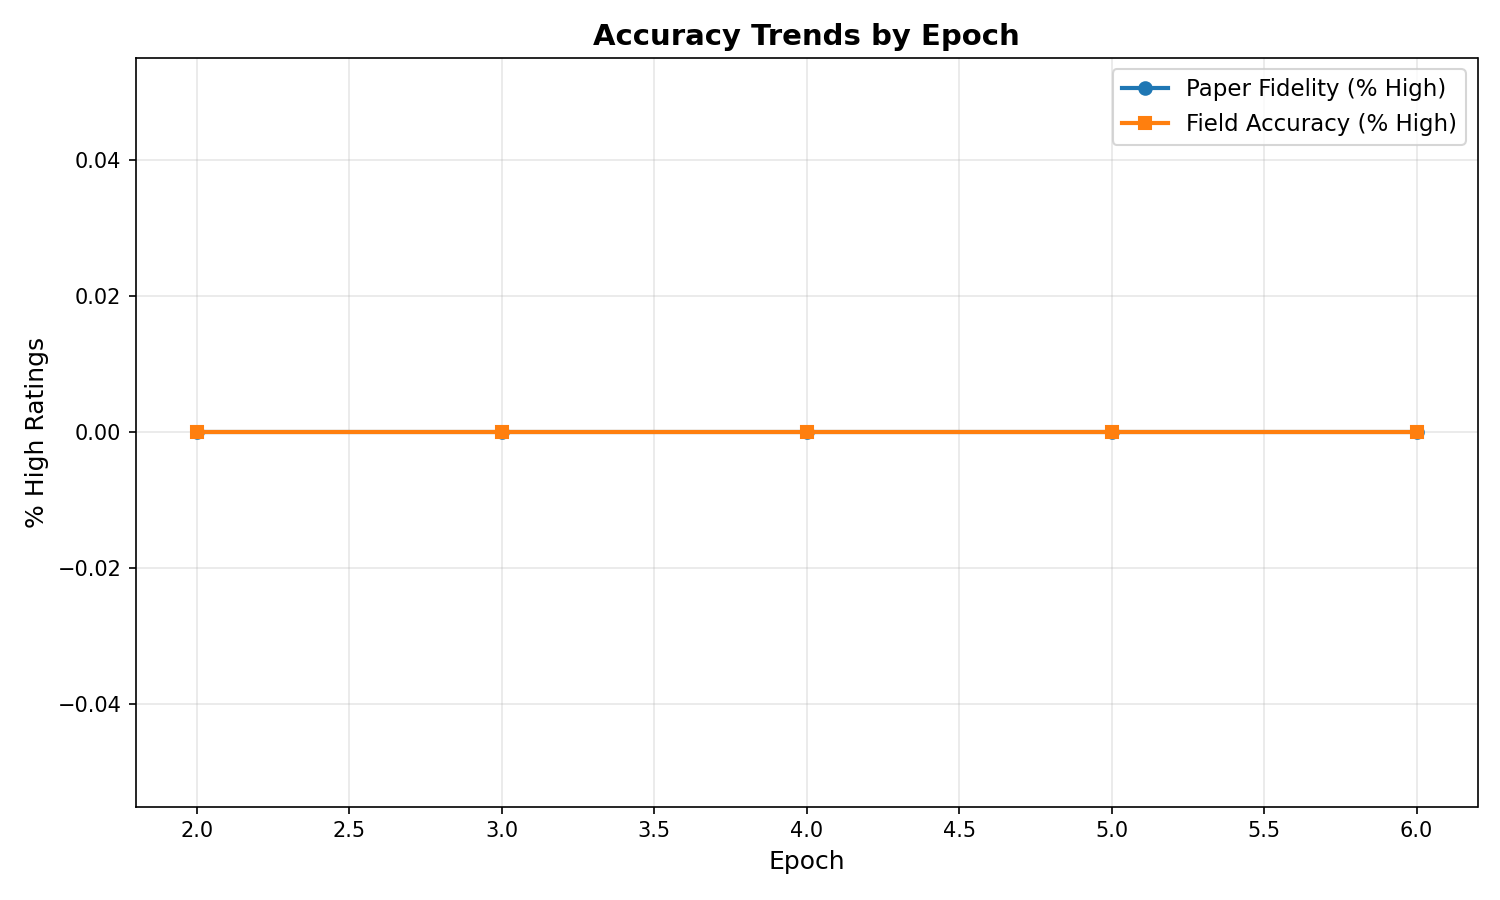
\includegraphics[width=0.95\linewidth]{epoch_fidelity_trends.png}
\caption{Paper Fidelity and Field Accuracy by Epoch. Shows declining accuracy in Epoch 6 relative to Epoch 5 across both dimensions. Epoch 6 contains 50.6\% of all citation units (273/539) and shows the largest accuracy declines.}
\label{fig:epoch_trends}
\end{figure}

\begin{figure}[H]
\centering
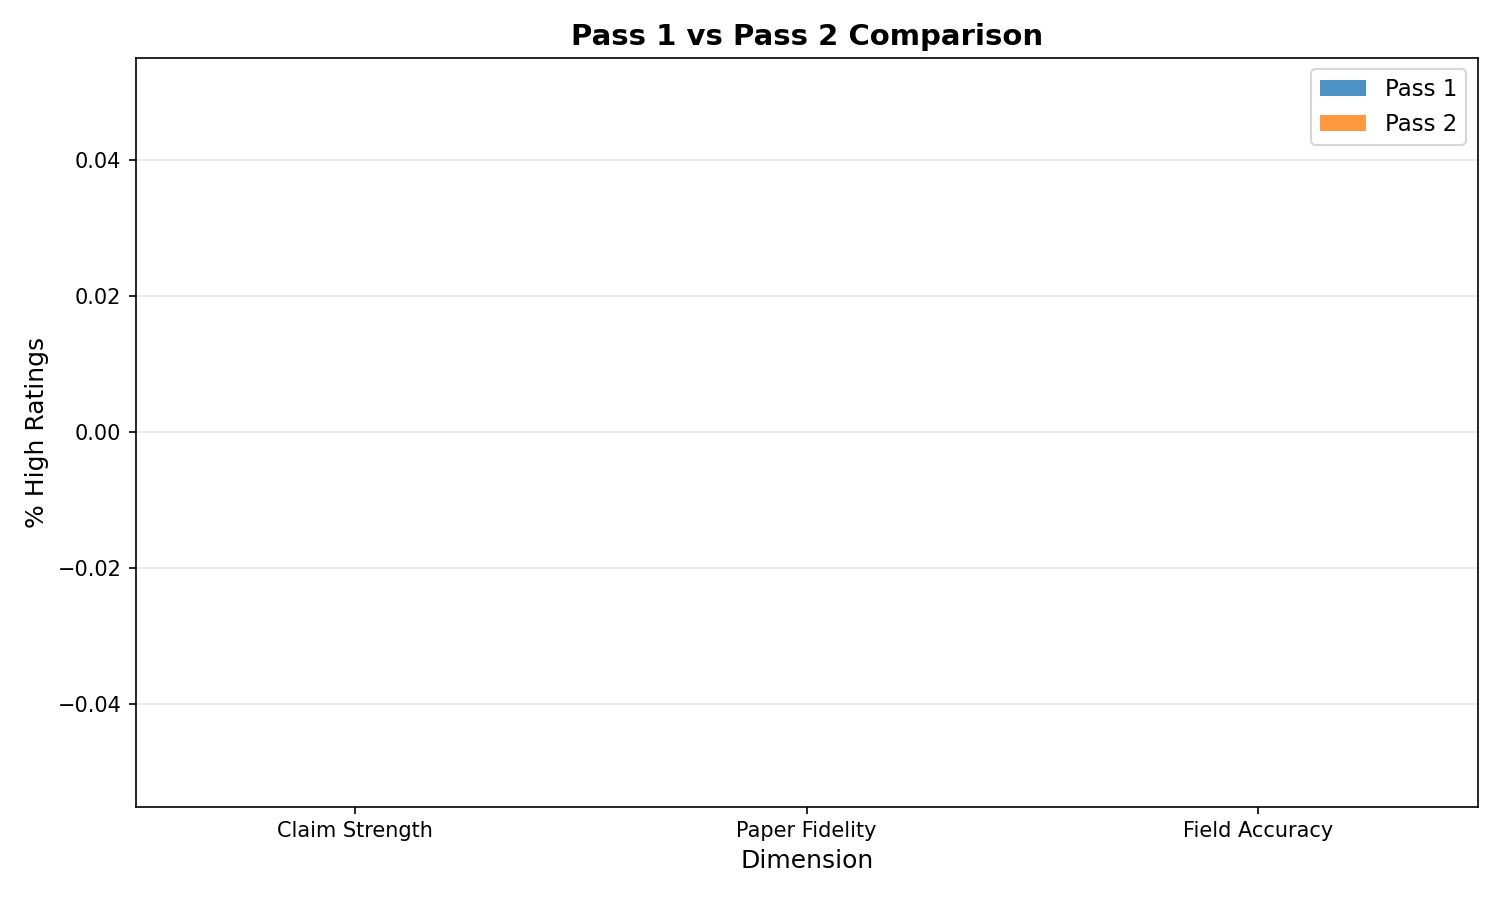
\includegraphics[width=0.95\linewidth]{twopass_comparison.png}
\caption{Two-Pass Coding Agreement. Exact agreement rates and Cohen's $\kappa$ values across three dimensions (Claim Strength, Paper Fidelity, Field Accuracy). Higher agreement suggests context changes interpretation less; lower agreement suggests context substantially affects coding.}
\label{fig:twopass}
\end{figure}

\begin{figure}[H]
\centering
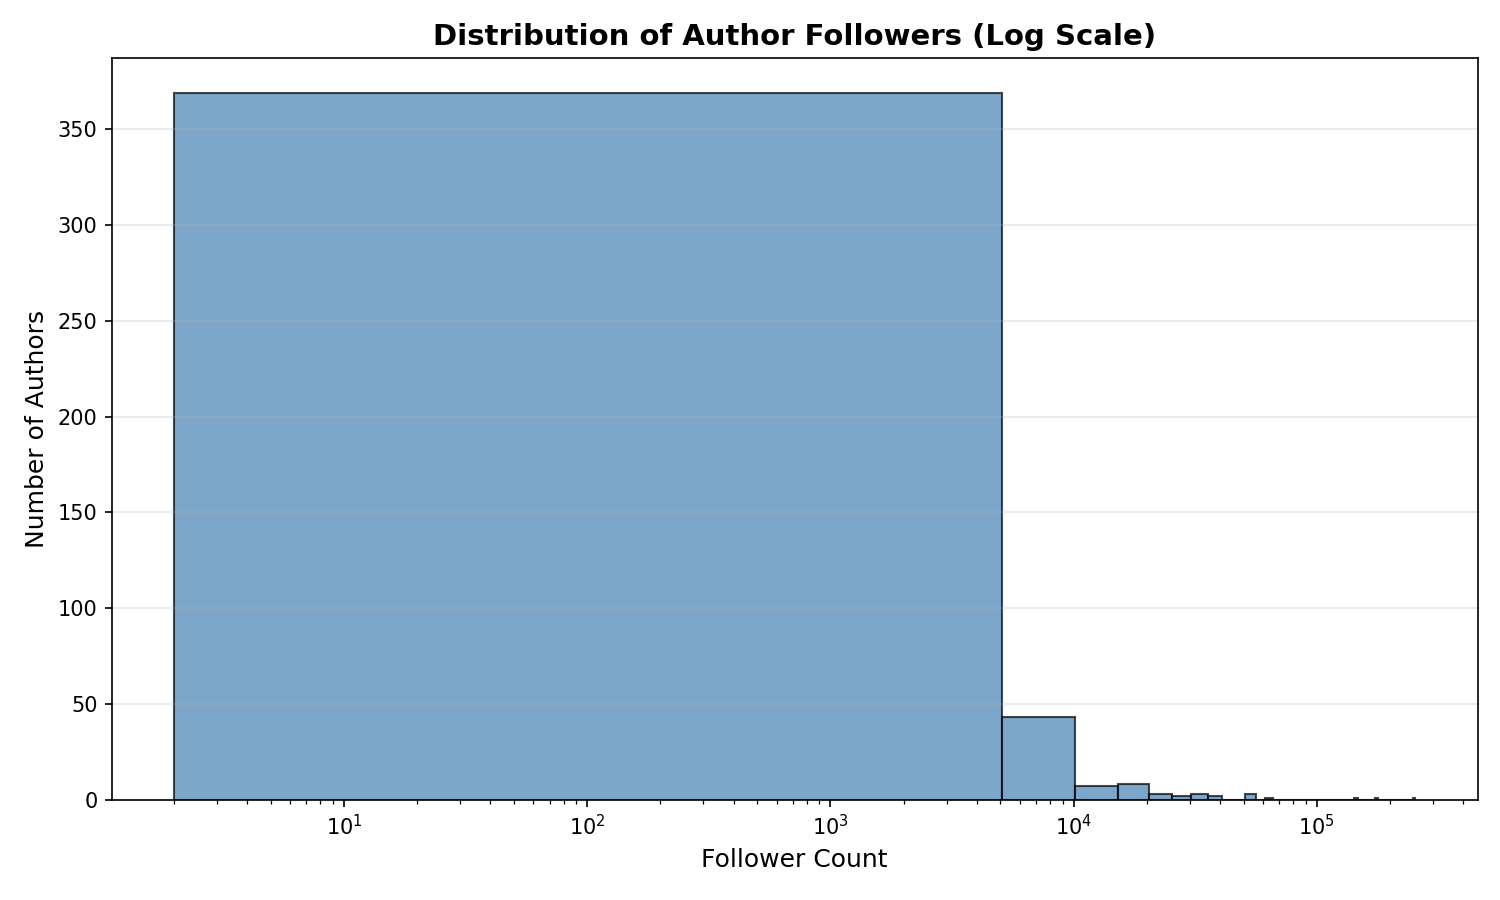
\includegraphics[width=0.95\linewidth]{author_followers_dist.png}
\caption{Author Follower Distribution. Heavy-tailed distribution (mean 4667, median 814) with a small number of highly-followed repeat citers. Insufficient variance for reach-accuracy correlation analysis.}
\label{fig:reach}
\end{figure}

\section{Table: Two-Pass Agreement Summary}

\begin{table}[H]
\centering
\small
\begin{tabularx}{\linewidth}{lrrrr}
\toprule
\textbf{Dimension} & \textbf{Exact Agree} & \textbf{Cohen's $\kappa$} & \textbf{Increased} & \textbf{Decreased} \\
\midrule
Claim Strength & 476/539 (88.3\%) & 0.695 & 49 (9.1\%) & 14 (2.6\%) \\
Paper Fidelity & 397/539 (73.7\%) & 0.551 & 65 (12.1\%) & 77 (14.3\%) \\
Field Accuracy & 398/539 (73.8\%) & 0.514 & 60 (11.1\%) & 81 (15.0\%) \\
\bottomrule
\end{tabularx}
\caption{Summary of two-pass (post-only vs.\ with-context) coding agreement. ``Increased'' refers to codes moving toward more generous/optimistic assessments; ``Decreased'' refers to codes moving toward more stringent assessments. The preponderance of ``Decreased'' codes for accuracy dimensions suggests context nudges coders toward more conservative evaluation.}
\label{tab:twopass}
\end{table}

\end{document}
